
En vrac, non trié.

===> Rajouter une intro de partie rappelant la nécéssité d'un simulateur ? (par manque de connaissance/documentation dans le domaine, etc...)

===> Enchaîner ensuite sur le fait qu'on doit pouvoir choisir les paramètres de simulation (pour pouvoir simuler des architectures variés, et même expérimentaux ou pour obtenir le suivi de certaines données particulières)

===> Comment on a implémenté cette entre-guillemets "modularité" -- comment l'utilisateur peut choisir ses paramètres (script Lua pour l'entrelacement, XML c'est déjà fait, etc...)

===> D'autres trucs sur l'implém, par exemple préciser ce que ne fait pas le simulateur (calcul de bande passante, prise en compte du prefetching) ???

===> Exemple d'entrée/sortie, comparaison de la sortie avec ceux obtenus avec d'autres logiciels (compteur hard) + graphes en fonction de la taille de l'entrée (pour voir s'il n'y a pas de déviation lorsqu'on a des programmes plus complexes)



\section{Cadre du simulateur}

Un simulateur est un programme qui va chercher à reproduire le fonctionnement de quelque chose. Un simulateur peut être nécessaire dans beaucoup de domaines. Par exemple, en météorologie, la simulation du mouvement des masses d'air permet de prévoir le temps avec des calculs probabilistes. C'est la même chose dans notre cas, nous voulons essayer de mesurer l'efficacité d'un programme sur différentes architectures de caches.

\subsection{Origine du projet}

La mémoire est un facteur de ralentissement des programmes très important de nos jours. Une mauvaise gestion de la mémoire peut être désastreux au niveau des performances, et pourtant, il n'existe pas de moyen efficace et précis de connaître l'utilisation de la mémoire au niveau des caches. Notre simulateur a pour objectif de pouvoir tester un programme ou un algorithme et d'observer le comportement des caches.

Les processeurs et les caches sont très optimisés par les constructeurs. La plupart des fonctionnalités sont connues, mais leur implémentation est gardée secrète. Pour connaître le fonctionnement des caches, il faut regarder la documentation pour savoir quels algorithmes sont implémentés.\\

Il existe des compteurs hardware qui permettent de connaître certaines statistiques sur les caches. Ces statistiques sont les données auxquelles il faudrait se rapprocher le plus. Elle ne sont cependant pas atteignable, les constructeurs optimisants un maximum les étapes. Par exemple, le prefetching permet de charger des lignes de caches en avance en fonction des accès mémoires courants du programme.

\subsection{Outils à disposition de l'utilisateur}

Les outils listés ci-dessous sont ceux utilisés par l'équipe de projet. Si d'autres outils offrent des fonctionnalités similaires, ils peuvent être utilisés en remplacement tant que les fichiers d'entrée du programme sont dans le bon format.

\paragraph{HWLoc}

est un logiciel qui permet de récupérer l'architecture des caches d'une machine. Il permet de générer un fichier xml que nous enrichissons. La paramétrisation de l'architecture des caches ne prend pas en compte les caches d'instructions, mais seulement les caches de données. L'utilisation de ce fichier est détaillé dans la section \ref{param_xml}.

\paragraph{MAQAO}

(Modular Assembly Quality Analyzer and Optimizer) est un outil d'analyse et d'optimisation de programmes. Nous n'utilisons qu'une fonctionnalité de MAQAO qui permet d'instrumenter un programme binaire afin de récupérer les opérations faites lors de l'exécution. Le paramétrage de MAQAO est effectué grâce à un fichier lua pour générer des traces de la forme voulue.

\subsection{Données simulées : analyses possibles des résultats}

--A finir ce soir--

\begin{lstlisting}
L3  basics     (misses:             6, hits:              0, writes_back:          0)
L2  basics     (misses:             6, hits:              0, writes_back:          0)
L1  basics     (misses:             4, hits:             44, writes_back:          1)
L1  basics     (misses:             6, hits:             42, writes_back:          2)
L2  basics     (misses:             0, hits:              0, writes_back:          0)
L1  basics     (misses:             0, hits:              0, writes_back:          0)
L1  basics     (misses:             0, hits:              0, writes_back:          0)
\end{lstlisting}

\section{Déroulement de la simulation}

--A finir ce soir--
Je voudrai faire un petit schéma pour montrer ça, c'est pas long à faire, ça sera cool et ça prendra de la place. Les sous sections du dessous se ressemblent un peu, faudra voir j'arrive à mettre quelque chose dedans sans faire de redites.

\subsection{Traitement d'une instruction : load/store}

\begin{lstlisting}
function interweave (current, nb_thread)
    i = i+1	 
    if i > sizeofblock then 
        i = 1 
        current = (current +1) % nb_thread
    end
    return current
end
\end{lstlisting}

--Explication de ce qu'il y a à l'intérieur des fonction load/store, application de la cohérence et remplacement--

Un des objectifs supplémentaire était d'optimiser la lecture des traces afin de gagner du temps sur les exécutions longues. Le format des traces actuel ne permet plus d'effectuer cela facilement, car il n'y a plus de boucles comme lors des premiers tests effectués. Cela est dû à MAQAO, qui ne peut pas à la fois optimiser la sortie avec des boucles \emph{for} et grouper les résultats pour chaque thread.

\subsection{Rapatriement prédictif d'une ligne}

--Je sais pas trop ce qu'il faut dire ici, c'est le fait que l'on considère que la donnée arrive quoi qu'il arrive ?--

\subsection{Mise à jour des lignes}

--Lister les différentes options disponibles offertes par les politiques et leurs applications, expliquer pourquoi--

La cohérence étant propre à un niveau de cache, elle peut être mise en place directement en considérant l'ensemble des caches de ce niveau. En réalité, les L1 ou les L2 n'intéreagissent pas toujours directement: s'ils ne sont pas reliés par un bus (cas du snooping), il faut passer par les niveaux haut dessus pour envoyer les messages. Cependant, la quantité de messages envoyés par cache pouvant être retrouvée à partir du nombre de \textit{misses} et de \textit{hits}, il n'est pas nécessaire de la calculer. \\

L'algorithme de cohérence (MSI, MESI, MOSI ou MOESI) est donc relativement facile à implémenter. Dans le cas du protocole MESI, il y a deux cas majeurs à gérer: \\
\begin{itemize}
\item Lorsqu'un cache fait un \textit{miss}, il parcours l'ensemble des autres caches pour savoir s'il doit mettre la donnée dans l'état E ou S. Dans le cas S, il modifie les données des autres caches pour quelles soient dans l'état S.
\item Quand un cache modifie une donnée qu'il avait dans l'état S, il invalide la donnée dans les autres caches.
\end{itemize}

\subsection{Problème d'ajout de ligne dans un cache plein}

--C'est limite expliquer les politiques et un peu la partie juste au dessus--

\subsection{\'Etapes de validation}
\begin{frame}
  \begin{block}{Pr\'esentation}
    \begin{itemize}
      \item Tests unitaires
      \item Validation durant le programme
      \item Comparaison avec des outils existants
      \item Benchmarks
    \end{itemize}
  \end{block}
  \begin{block}{Premiers outils de v\'erification}
    \begin{itemize}
      \item Validation des politiques basiques
      \item Validation du comportement inclusif
      \item Utilisation de \textsf{PAPI}
    \end{itemize}
  \end{block}
\end{frame}

\begin{frame}{Benchmarks basiques}
\begin{figure}[H]
   \begin{minipage}[l]{.46\textwidth}
     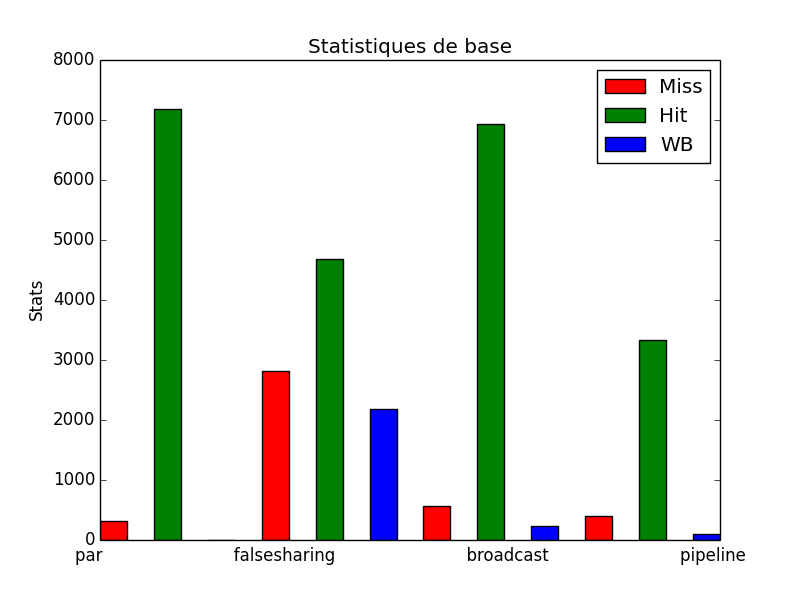
\includegraphics[scale=0.22]{images/stats_L1.png}
   \end{minipage} \hfill
   \begin{minipage}[r]{.46\textwidth}
     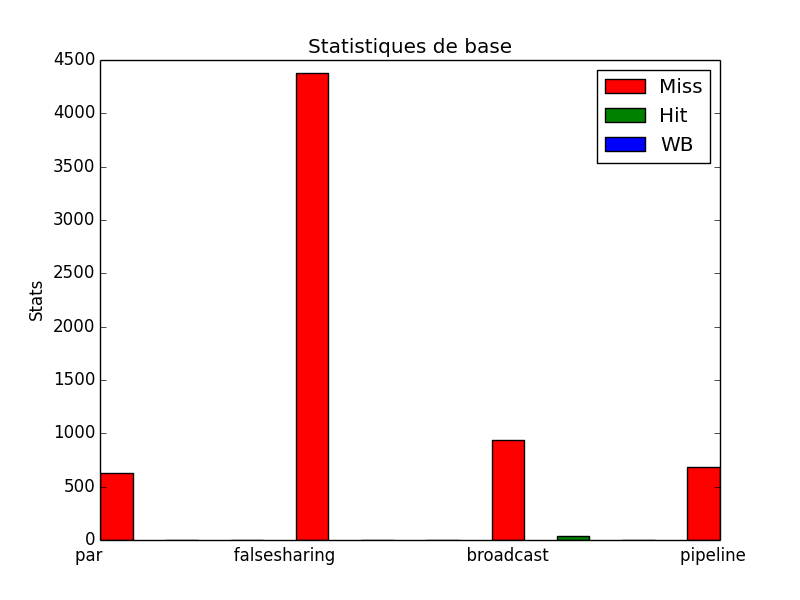
\includegraphics[scale=0.22]{images/stats_L2.png}
   \end{minipage}
\end{figure}

\begin{figure}[t!]
  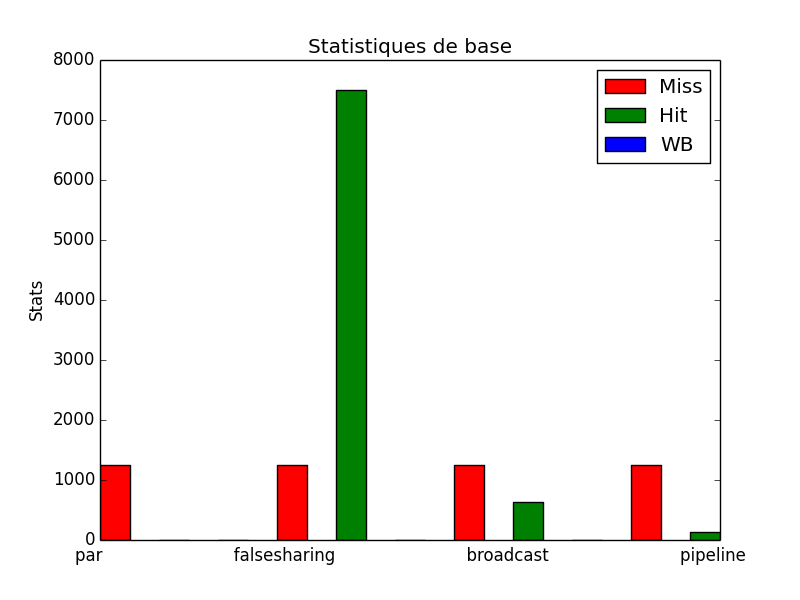
\includegraphics[scale=0.22]{images/stats_L3.png}
\end{figure}
\end{frame}

\begin{frame}{Benchmarks avanc\'es}
\begin{figure}[H]
   \begin{minipage}[l]{.46\textwidth}
     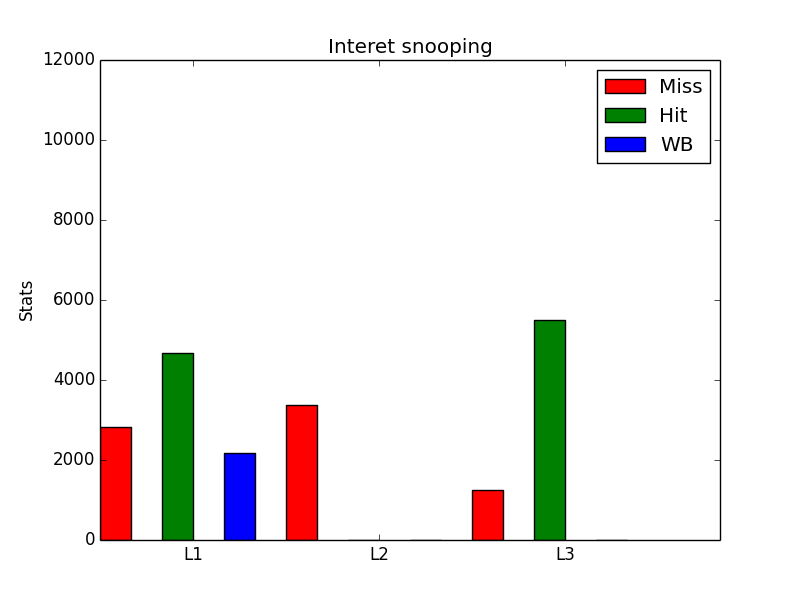
\includegraphics[scale=0.22]{images/stats_falsesharing_snooping.png}
   \end{minipage} \hfill
   \begin{minipage}[r]{.46\textwidth}
     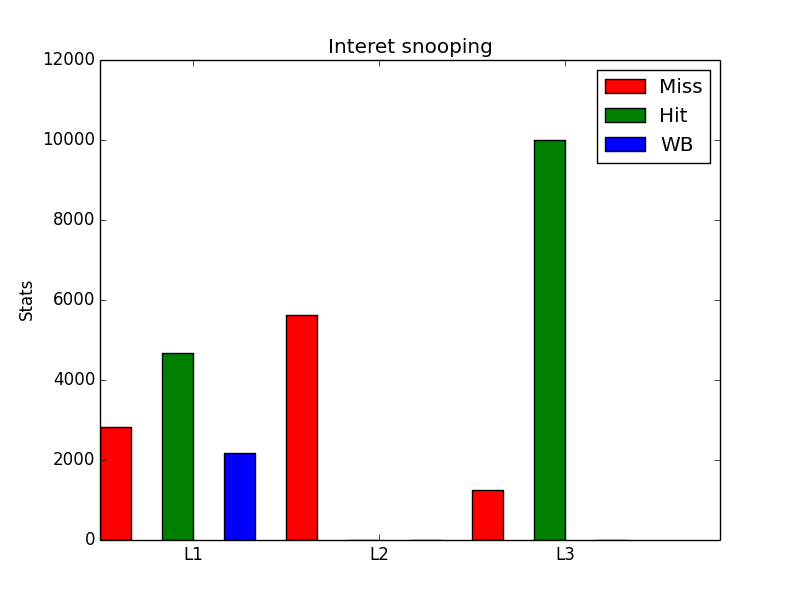
\includegraphics[scale=0.22]{images/stats_falsesharing_no_snooping.png}
   \end{minipage}
\end{figure}
  \begin{block}{Autres benchmarks}
    \begin{itemize}
      \item \emph{Directory manager}
      \item Politiques de coh\'erence MSI vs MESI
      \item Scalabilit\'e
    \end{itemize}
  \end{block}
\end{frame}

\subsection{Limites \`a  propos de la simulation des caches}
\begin{frame}
  \begin{block}{Probl\`emes li\'es aux architectures multi-c{\oe}ur}
    \begin{itemize}
      \item \textsf{prefetching}
      \item synchronisations
      \item changements de contextes 
    \end{itemize}
  \end{block}
  \begin{block}{Limites de \textsf{Cassis}}
    \begin{itemize}
      \item bande passante non mod\'elis\'ee
      \item \textsf{Directory manager} basiquement mod\'elis\'es
      \item statistiques non calibr\'ees avec des benchmarks classiques
      \item utilisation de m\'etriques non usuelles
    \end{itemize}
  \end{block}
\end{frame}


\section*{Conclusion}
\begin{frame}
  \begin{block}{Objectifs atteints}
    \begin{itemize}
      \item Cahier des charges respect\'e
      \item Param\'etrisation compl\`ete
    \end{itemize}
  \end{block}

  \begin{block}{\'Evolution possible}
    \begin{itemize}
      \item Complage avec un simulateur \textsf{on-line}?
      \item Utilisation de benchmarks pour calibrer les r\'esultats?
    \end{itemize}
  \end{block}
\end{frame}

%\section{Validation de la simulation}
%
%Le simulateur ressort des statistiques qui se doivent d'être correcte. Une des grandes difficultés de ce logiciel est de vérifier la justesse de ces statistiques.
%
%\subsection{Tests unitaires}
%
%Des tests unitaires sont effectués pour vérfifier le bon fonctionnement du programme. Les tests portent sur les parties critiques du code, à savoir le chargement d'une architecture ainsi que les politiques de cohérence et de remplacement des données.
%
%\subsection{Validation comparative}
%
%Afin de s'assurer que les politiques de cohérence fonctionnaient, des tests de comparaison sur un petit nombre d'opérations (moins de dix) furent entrepris avec les résultats théoriques attendus. Ces tests ont permis dans un premier temps de valider le code dans le cas où les caches sont vides. Cependant, ces valisations sont fastidieuse et le simulateur doit fonctionner pour un très grand nombre d'opération. Comme on ne peut avoir de vérifications exactes, la validation des résultats a pu se faire grâce à d'autres logiciels.\\
%
%Dans un premier temps, le logiciel PAPI (Performance Application Programming Interface) permet d'utiliser les compteurs hardware. Ces compteurs comportent plusieurs problèmes. Le premier point est qu'il ne sont très dépendant des machines. Les compteurs peuvent être très différents d'une machine à une autre, ou ne sont pas toujours activés. Le second point vient du fait que l'on obtient les opérations exactes de la mémoire. Ces opérations prennent en compte un trop grand nombre d'optimisations pour être simulée facilement.\\
%
%--Mettre des chiffres pour PAPI ?--
%
%Dans un second temps, nous avons effectué des tests avec le logiciel valgrind (logiciel de débogage pas à pas), plus précisement le module nommé cachegrind qui permet d'observer les opérations sur la mémoire lors de l'exécution d'un programme.
%--Je sais pas trop ce qu'il s'est passé avec cachegrind--
%
%\subsection{Benchmarks}
%
%Des benchmarks ont été mis en place pour tester le schmilblick.
